\chapter{Transfer Learning}\label{Tl}
In this chapter, the technique of transfer learning will be introduced.
It can be considered as a broad interpretation of related work.\\
This chapter is organized as follows:    
First of all, we discuss some challenges of traditional machine learning algorithms.
Furthermore, some real world and machine learning sample problems are discussed.\\
In the second section, the task transfer learning in the context of classification will be described.\\
There are various definitions of transfer learning in general.
Many of the solutions obtained in this chapter are made for different definitions.
Moreover, because of this the difficulty of the problem which is solved by the solutions may vary, see \ref{TlSecDef}.\\
Additionally, we will see how the difference in transfer learning is measured.\\
Then, the settings of transfer learning will be introduced.
The settings are implying the different setups to solve the transfer problem.\\
In the next section, the two main types of the transfer learning, which describe the conditions of feature space and probability distributions, will be introduced and explained.
These types can be divided into approach-categories.
Most of the discussed solutions are based on the formal ideas of a category.\\
The section, negative transfer deals with the problem that the provided transfer learning solutions are in fact worse than the baseline methods.
For details to kernels see section \ref{EmSubSecKernel}.

\section{Challenges of Supervised Learning Algorithms}\label{TlSecChal}
The current state of 'traditional' supervised learning algorithms is the assumption that training and test data existing in the same feature space and that they have the same distribution.
They are successfully learning patterns and predict events in the future.
However, it is not always possible to obtain training and test data, which matches in distribution or features space.
A reason for this is that training data, which has to be labeled, is expensive or difficult to achieve.\cite[p. 1]{Weiss.2016}\\
When it comes to supervised learning, the algorithms are designed in a way to learn from the pre-labeled data and hence it is crucial for this types of algorithms to have some.\cite[p. 6-7]{Theodoridis.2008}\\
In the 'traditional' manner, which applies to the most statistical models, to solve the problem of differences, one has to collect new training data for the new feature space or distribution of the test data and rebuild the model.\cite{Pan.2010}
Therefore, the good performance cannot be obtained, when the training and test data differs in feature space or distribution.
This is the reason, one has to find a classifier, which can be applied to the target domain, although it is trained on the source domain
This is the main motivation of Transfer Learning.\cite[p. 1.]{Weiss.2016}\\
A simple interpretation of Transfer Learning in the real world is given in the following:
Imaging two people, who want to learn the piano.
One has never played any musical instrument before, while the second one has previous knowledge on how to play the music through experience with other instruments.
The latter will be able to learn the new instrument much faster than the first one with no previous experience because he can transfer his general music knowledge to boost his learning of the new instrument.\cite[p. 1]{Weiss.2016}\\
When going back to machine learning, there are more technical examples.
Consider the task of web document classification.
The goal is to classify web documents in predefined categories.
The training data in this example are university web pages, which are associated with a category by manual labeling.
If we want to classify our test data, which does not come from a university page, then the data features or distribution is different, based on the structure or topics of the new web pages.
Therefore, we can not directly apply the classifier trained on the university web pages and assume a good category prediction rate on non-university web pages.
Instead, we have to collect new websites from the same type as of the test web pages, assign the category manually and finally learn a new model.
This process could be avoided if a classifier could transfer knowledge from one domain of pages into another web page domain.\cite{Pan.2010}\\
The last example is given from the topic of product reviews.
Consider the problem that a model needs to be learned, in a way that it can automatically classify positive and negative reviews on a product.
To create a source domain, one has to collect many reviews of the product and manually decide if it is positive or negative.
Then the model can be trained and predict the sentiment of new reviews.
However, if the product changes, then the distribution of the review may change, and the traditionally learned classifier cannot be applied anymore.
Therefore, again one has to collect reviews manually and annotate them.
This can be a very expensive process, and therefore the learner should be adaptable so that it can be learned on the source domain (one product category) and can help to learn the classification model (another product category).\cite{Pan.2010}

\section{Definition of Transfer Learning}\label{TlSecDef}
\begin{figure}
	\centering
	\begin{subfigure}{.5\textwidth}
		\centering
		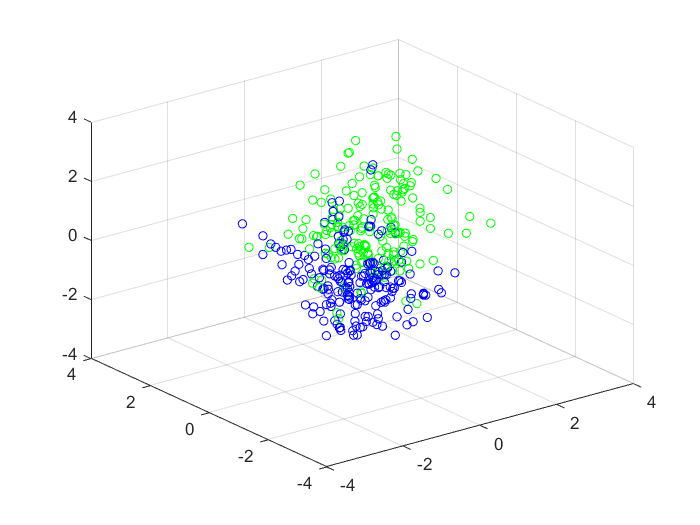
\includegraphics[width=1\linewidth]{figures/TraditionalProblem.png}
		\caption{Traditional Learning Problem\label{FigTradProblem}}
	\end{subfigure}%
	\begin{subfigure}{.5\textwidth}
		\centering
		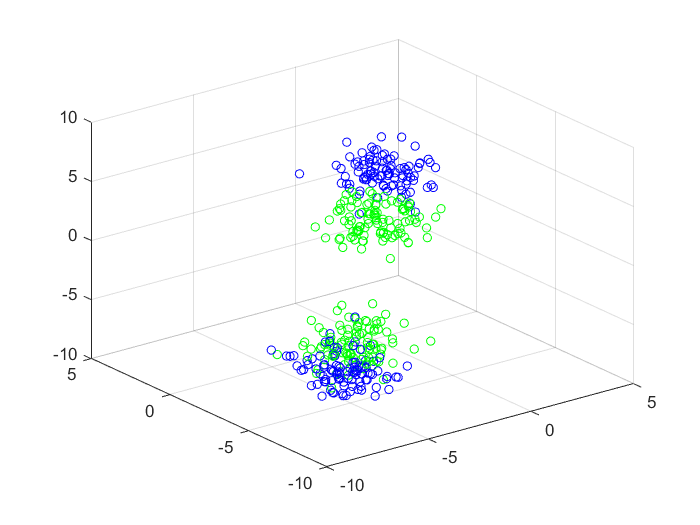
\includegraphics[width=1\linewidth]{figures/TransferProblem.png}
		\caption{Transfer Learning Problem \label{FigTLProblem}}
	\end{subfigure}
	\caption[Comparison of Transfer and Traditional Learning Problems]{The figures show the comparison of distributions for two classes in the traditional and the transfer learning state. The left shows one domain with where the classes are similarly distributed. The right figure shows two different domains with different marginal and conditional probability distributions.\label{FigProblemComparison}}
\end{figure}
Now that more practical examples have been given, the term transfer learning and associated keywords are defined in this section.\newline
In this thesis, a domain $\mathcal{D}$ is composed of a $D$-dimensional feature space $\mathcal{F}$, which can be feature extraction a of text documents. Moreover, a marginal probability distribution of a data matrix $\mathbf{X}$ is denoted with  $P(\mathbf{X})$.
Formally, this means $\mathcal{D} = \{\mathcal{F},P(\mathbf{X})\}$ with $\mathbf{X} \in \mathcal{F}$.
In general, if two domains $\mathcal{X}$ and $\mathcal{Z}$ are different, then they have either different feature spaces or marginal distributions.\\
This can be expressed as $\mathcal{F_{Z}} \neq \mathcal{F_{X}} \vee P(x) \neq \textit{P}(z)$.\cite[p. 542]{Aggarwal.2015}
The issue of different distributions is illustrated in figure \ref{FigProblemComparison}.
In \ref{FigTradProblem} the traditional problem with similar source and target probability distributions is shown.
The figure \ref{FigTLProblem} shows the problem of transfer learning where conditional and marginal probability distributions are different (two domains).
The samples are generated with the Gaussian-Random function in MatLab.
The blue and green colors are showing two classes.
Moreover, \ref{FigTLProblem} shows the problem with two domains.\\
A task $\mathcal{T}$ with a given domain $\mathcal{D}$ is put together with a label set $\mathcal{Y}$, for example $\{-1,1\}$, and a classifier $f(\cdot)$ which is  $\mathcal{T} = \{\mathcal{Y},\textit{f}(\cdot)\}$ with $\mathbf{y} \in \mathcal{Y}$.
The vector $\mathbf{y}$ represent the (predicted) labels for \textit{all} data points regarding the label set $\mathcal{Y}$.
The function $f(\cdot)$ is a predictive function to make predictions for unseen, i.\,g. new data points $\mathbf{x}$.
From a probabilistic viewpoint we can interpret $f(\mathbf{x})$ as $P(y\mid \mathbf{x})$.
In other words, given $\mathbf{x}$ how probable it is that label y is correctly assigned.
For example, based on the content of a document, how probable it is to be correctly assigned to certain category.\cite[p. 542]{Aggarwal.2015}\\
In classification, the number of varying labels will distinguish the classification problem.
The Binary classification problem for two labels, e.\,g. $\mathcal{Y} ={-1,+1}$ or discrete values, i.\,e. multiple classes, for example $\mathcal{Y}= \{1,2,..,C\}$ with $C$ classes.
In general, two tasks $\mathcal{T_X}$ and $\mathcal{T_{Z}}$ are different if they have varying conditional probability distributions or label spaces, which means $\mathcal{Y_{X}} \neq \mathcal{Y_{Z}} \vee P(y\mid \mathbf{x}) \neq P(y\mid \mathbf{z})$.\cite[p. 542]{Aggarwal.2015}\\ 
Note that in this thesis if we talk about transfer learning, then the training domain is denoted as $\mathcal{Z}$ and $\mathcal{X}$ represents the test domain.
For the binary case within transfer learning the following definitions are made:
Consider $\mathcal{D_Z} = \{(\mathbf{z}_i,y_{\mathcal{Z}i})\}_{i=1}^{N}$ as source domain data where $\mathbf{z}_i \in \mathcal{F}_\mathcal{Z}$ as a single observation, for example, one document in the feature space. It is part of the training data matrix and therefore is part of $P(\mathbf{Z})$.
Moreover, $y_{\mathcal{Z}i} \in \mathcal{Y}_\mathcal{Z}$ is the corresponding class label, which forms the whole N sized label vector $\mathbf{y}_\mathcal{Z}$.
Additionally, the target domain data $\mathcal{D_X} = \{(\mathbf{x}_i,y_{\mathcal{X}i})\}_{i=1}^{M}$.
Analogue, $\mathbf{x}_i$ is a single observation with $\mathbf{x}_i \in \mathcal{F}_\mathcal{X}$ and the corresponding class label $y_{\mathcal{X}i} \in \mathcal{Y}_\mathcal{X}$, which is again summarized as $M$ sized training vector $\mathbf{y}_\mathcal{X}$.\cite[p. 2]{Aggarwal.2015}\\
Note that we are doing the assumption that our problem has by default more than one dimension and therefore we write a single observation as a vector of features.
Because of this, the whole data is represented as a matrix.
\begin{mDef}[Transfer Learning]\label{DefTl}
	Given a source domain $\mathcal{Z}$ and learning task $\mathcal{T}_\mathcal{Z}$, a target domain $\mathcal{X}$ and learning task $\mathcal{T}_\mathcal{X}$, transfer learning aims to help improve the learning of the target predictive function $f_\mathcal{X}(\cdot)$ in $\mathcal{X}$ using the knowledge in $\mathcal{Z}$ and $\mathcal{T}_\mathcal{Z}$, where $\mathcal{Z} \neq \mathcal{X}$, or $\mathcal{T}_\mathcal{Z} \neq \mathcal{T}_\mathcal{X}$.\cite[p. 542]{Aggarwal.2015}	
\end{mDef}
Summarizing, our source domain consists of $\mathcal{Z}=\{\mathcal{F}_\mathcal{Z},P(\mathbf{Z})\}$ and task $\mathcal{T_Z}=\{\mathcal{Y_Z},f_\mathcal{Z}(\mathbf{Z})\}$ with $f_\mathcal{Z}(\mathbf{Z}) = P(\mathbf{y}_\mathcal{Z}|\mathbf{Z})$. Moreover, the target domain is  $\mathcal{X}=\{\mathcal{F}_\mathcal{X},P(\mathbf{X})\}$ and $\mathcal{T_X}=\{\mathcal{Y_X},f_\mathcal{X}(\mathbf{X})\}$ with $f_\mathcal{X}(\mathbf{X}) = P(\mathbf{y}_\mathcal{X}|\mathbf{X})$. 
If we consider that the training and testing domain are equal and their learning tasks are the same, we step back to the traditional machine learning problem.
Note that in this thesis the size of the whole dataset (source and target data points) is denoted as $K=N+M$.
Furthermore, if any of the methods are transforming the original features into a subspace. The dimension of the subspace is denoted with $L$.
The notation is summarized in appendix \ref{appaA} table \ref{ATableNotation}.\\
According to our challenges from section \ref{TlSecChal}, the definition can be explained with the help of the web document classification example.\cite[p. 4]{Weiss.2016}
The example can be divided into two cases:
In case one, if two domains are different, which means that $\mathcal{Z} \neq \mathcal{X}$ as above, then they differ either the feature space $\mathcal{F_Z}, \neq \mathcal{F_X}$ or in their marginal probability distribution $P(\mathbf{Z}) \neq P(\mathbf{X})$.
Going back to the web document example, the first would imply that the language of the two documents is different.
The second could be caused by the fact that the documents are focusing on various topics, which would be lead to different term features.\cite{Pan.2010}\\
The second case is that the tasks are different, which implies $\mathcal{T_Z} \neq \mathcal{T_X}$ and can further be divided that they rather differ in the label space $\mathcal{Y_Z} \neq \mathcal{Y_X}$ or the conditional probability of the two tasks are different with $P(\mathbf{y}_\mathcal{Z}\vert \mathbf{Z}) \neq P(\mathbf{y}_\mathcal{X}\vert \mathbf{X})$.
In practice, the first would imply that the source task has only two categories, which results in a binary classification problem, although the target task has more than two labels and is, therefore, a multi-class problem.
The second case could be based on the fact that source and target documents are divided into very unbalanced user-defined classes.
Finally, if there exists any relation between the feature spaces of the two domains, then they are \textit{related}.\cite{Pan.2010}\\
Note that in the context of transfer learning the term \ac{DA} may appear.
Based on the discussion in \cite{Pan.2011}, the following definition can be extracted.
\begin{mDef}[Domain Adaptation]\label{DefDa}
	Given a source domain $\mathcal{Z}=\{\mathcal{F}_\mathcal{Z},P(\mathbf{Z})\}$ and learning task $\mathcal{T_Z}$ and a target domain $\mathcal{X}=\{\mathcal{F}_\mathcal{X},P(\mathbf{X})\}$ and learning task $\mathcal{T_X}$. Let $\mathcal{T_Z} = \mathcal{T_X}$ and the domains $\mathcal{Z} \neq \mathcal{X}$ in a way that $\mathcal{F}_\mathcal{Z} = \mathcal{F}_\mathcal{X}$ and $P(\mathbf{Z}) \neq P(\mathbf{X})$, domain adaptation aims to help improve the learning of the target predictive function $f_\mathcal{X}(\cdot)$ in $\mathcal{X}$ using the knowledge in $\mathcal{Z}$.
\end{mDef}
This is related to the covariance shift problem.\cite{Pan.2011}
It assumes that the domain data generation is made in a way that the sampling, which the data is based on, is $P(\mathbf{y}\vert \mathbf{X})P(\mathbf{X})$.
Furthermore, the marginal distribution $P(\mathbf{X})$ changes through the domain shift that the marginal distribution for data sampling of the source and target data are different. As a consequence, the distributions are different.\cite[p. 8-9]{QuinoneroCandela.2009}\\
In practice, we can observe that the key challenge of \acl{DA} methods is to focus on aligning the differences in the marginal distribution, which can be observed in \cite{Pan.2011}, \cite{Long.}, \cite{Fernando.}, \cite{Arnold.2007} and \cite{Pan.2011}.

\FloatBarrier
\section{Measurement of Difference}\label{TlSecMeasure}
From the previous examples in \ref{TlSecChal} and definitions in \ref{TlSecDef}, it seems that the domains are different.
This difference needs to be determined to classify the amount of transfer which is done.
In this thesis, it is measured with the \ac{MMD} and \ac{KLD}.
Note that they only consider the differences in the marginal probability distributions.
Another, point worth mentioning is that the methods, which we will introduce later on, are based on these measures.
For example, the \acl{TCA} and the \acl{JDA} solutions are using the \acs{MMD} in their optimization problems.
On the other hand, the authors of TrAdaBoost using the \acs{KLD} to determine the difference in domains, to measure the quality of the transfer-algorithm.\cite{Long.}\cite{Pan.2011}\cite{Dai.}
\subsection{Maximum Mean Discrepancy}\label{TlSubSecMMD}
First, the \acl{MMD} is a non-parametric function to measure the difference of two \ac{IID} samples $\mathbf{X}$ and $\mathbf{Y}$ drawn from p and q respectively, which is introduced by \cite[p. 724-728]{Gretton.2012}.\\
Two samples of a random variable are independent if a current sample is not influenced by any previous samples and will not influence following samples.
Identically  distributed, as the name says, requires that the random variables are must have the same distribution.\cite[p. 7-8]{Czado.2011}\\
The \acs{MMD} is calculated with samples drawn from two distributions.
It measures the distance between the expectations of two samples, $\textbf{X}=\{x_1,...x_N\}$ and $\textbf{Y}=\{y_1,...y_M\}$
in a \ac{RKHS} $\mathcal{H}$.
Assuming that $\mathbf{X} \sim p$ and $\mathbf{Y} \sim q$.
Because $\mathcal{H}$ is a Hilbert space, the mapping function is defined as $f(x) = \langle f,\phi(x) \rangle_\mathcal{H}$ with $\phi(x) = k(x,\cdot)$ as positive semi-definite kernel.
Note that a \ac{PSD} kernel, has only non-negative eigenvalues.\cite[p. 30]{Scholkopf.2001}\\
With the use of the \acs{RKHS} the authors claim, that the $f(\cdot)$ is smooth and therefore the \acs{MMD} it is. 
Moreover, the \acs{MMD} is easily expendable, for example, with new points drawn from $p$ and $q$.
Finally, the \acs{MMD} and his empirical estimation are defined as \eqref{EqMMdExp} and \eqref{EqMMdExpEm}:\cite[p. 726-727]{Gretton.2012}
\begin{equation}\label{EqMMdExp}
MMD[p,q]^2:=\big[sup(E_{p}[f(x)] - E_{ q}[f(y)])\big]^2
\end{equation}
\begin{equation}\label{EqMMdExpEm}
MMD_e[\mathbf{X},\mathbf{Y}]:= \abs{\frac{1}{M}\sum_{i=1}^{M}f(\mathbf{x}_i) - \frac{1}{N}\sum_{i=1}^{M}f(\mathbf{y}_i)}
\end{equation}
Note that $f(\cdot)$ is the kernel function.
Furthermore, the empirical \acs{MMD} is biased.
If $p$ and $q$ both are equal probability distributions, respectively $p = q$, then \ac{MMD}\textsubscript{e} = 0.\cite[p. 726-727]{Gretton.2012}\\
The \acs{MMD} is symmetric after it takes the absolute value, as shown in \eqref{EqMMdExpEm}.\\
Another advantage of \eqref{EqMMdExpEm} is that it can be calculated based on samples.
Unlike the following Kullback-Leibler Divergence where the density has to be estimated before, the \acs{KLD} can be calculated.\cite{Long.2015}\\
The code for the \acs{MMD} estimation can be obtained from the website of the Gatsby Computational Neuroscience Unit\footnote{\url{http://www.gatsby.ucl.ac.uk/~gretton/mmd/mmd.htm}}, which uses the standard Gaussian kernel for feature mapping.

\subsection{Kullback-Leibler Divergence}\label{TlSubSecKLD}
The \acl{KLD} is also named Kullback-Leibler-Risk.
It needs two probability distributions f and g of a random Variable X.
For discrete variables $x_i, i=1,..,M$ with $p_i=f(x_i)$ and $q_i=g(x_i)$ as probabilities respectively, the \acs{KLD} is calculated as:\cite[p.5-7]{Commenges.}
\begin{equation}
KL(g\mid f) = \sum_{i=1}^{M}p_i\log\frac{p_i}{q_i}
\end{equation} 
For continues variables the \ac{KLD} is computed:
\begin{equation}
KL(g\mid f) = \int f(x)log\frac{f(x)}{g(x)} dx
\end{equation}
For all f and g it is $KL(g\mid f) \ge 0$. Next, $KL(f\mid f) = 0$ and finally, if $KL(g\mid f) = 0$, then $f = g$, which implies that the two distribution are nearly the same.
Note that the \acs{KLD} is not symmetric and as a consequence the  switch of variables will result in another \acs{KLD}\cite[p.5-7]{Commenges.}\\
Because the density has to be estimated, the \acs{KLD} in this thesis will be determined by a Bayesian method approach, which is described in the supplementary material of \cite{Berkes.2011}.
The source code for the \acs{KLD} estimation can be found on GitHub\footnote{\url{https://github.com/pberkes/neuro-kl}}.

\section{Settings of Transfer Learning}\label{DefTlSecSett} %
In this section, the different settings of transfer learning are proposed.
There are various settings of the transfer learning definition, which specifies the composition of domains and tasks and how they are related to each other.
Therefore, each setting has his requirements on how labeled data in the source and target domain is available.
In general, the settings could be summarized with 'What to transfer?' and 'How to transfer?'.
The various settings are related to some traditional machine learning task.\cite{Pan.2010}\\
As we will see in the following, the definitions of homogeneous (\ref{TlSecHomo}) and heterogeneous (\ref{TlSecHetero}) transfer learning and the definitions of the settings will overlap.\cite[p. 5-6]{Weiss.2016}\\
In general, we will stick to the definitions of homogeneous and heterogeneous, because these are more general in comparison with the settings.
Therefore, the settings are used to express the categories of the transfer learning methods more precisely.
Additionally, but more importantly, we want to focus on the fact, whether labeled or unlabeled target data are required for the knowledge transfer.
The practical methods will be explained within the section of homogeneous and heterogeneous transfer learning.
The relationship is shown in figure \ref{FigSettingsTransferLearning}.
\begin{figure}
	\centering
	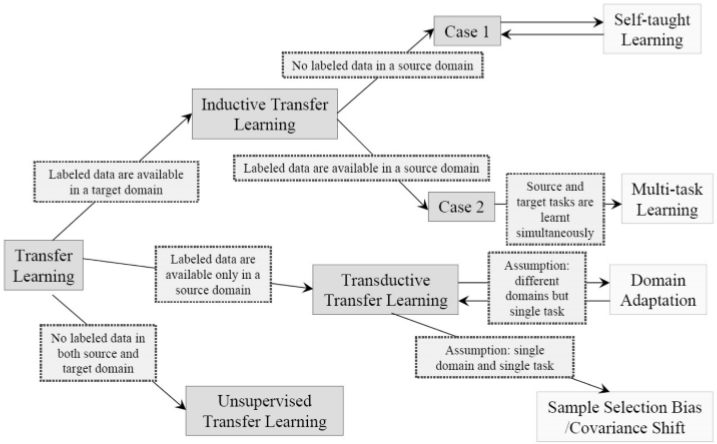
\includegraphics[width=.8\linewidth]{figures/SettingsTransferLearning.png}
	\caption[Settings of Transfer Learning]{This figure shows the various settings for transfer learning and their relation to traditional machine learning or sampling problems. Moreover, the figure shows the required dataset compositions regarding unlabeled or labeled target data.\cite{Pan.2010}}
	\label{FigSettingsTransferLearning}
\end{figure}

\subsection{Inductive-Transfer Learning}\label{TlSubSecInduc}
The setting \ac{ITL} makes the assumption that source task and target task are different, regardless of whether the domains of source and target are different or not.
Methods of this setting requiring some labeled test data to \textit{induce} a predictive model $f_\mathcal{X}(\mathbf{X})$ for the training domain.\cite{Pan.2010}
Therefore, Pan et al. formulated the following definitions.
\begin{mDef}[Inductive Transfer learning {\cite{Pan.2010}}]\label{DefITL}
	 Given a source domain $\mathcal{Z}$ and a learning task $\mathcal{T_Z}$, a target domain $\mathcal{X}$ and a learning task $\mathcal{T_X}$, inductive transfer learning aims to help improve the learning of the target predictive function $f_\mathcal{X}(\cdot)$ in $\mathcal{X}$ using the knowledge in $\mathcal{Z}$ and $\mathcal{T_Z}$, where $\mathcal{T_Z} \neq \mathcal{T_X}$, while some labeled target domain data is available.
\end{mDef} 
With this in mind, there are in fact two special cases to consider.
The first one tries to achieve high performance in the target task by requiring not only some labeled test data but lots of labeled training data.
This is related to the multi-task learning approach where a learner tries to learn both domains, the source and target domain,  simultaneously.\cite{Pan.2010}\\
In the second case, there is no labeled source data at all available.
The goal is similar to the self-thought learning setting.
The challenge of self-thought learning is that information from the source domain can not be applied to the target because they are not the same and therefore can not be used directly.
Summarizing, because the source data cannot be used directly, we have to find parts of the data which can be combined with a few labeled target data to reach the goal.\cite{Pan.2010}\\
In the section \ref{TlSubSecInstance}, we will give an example of an instance based approach, based on the inductive transfer learning setting.
Note that this solution tries to align the marginal distributions with some labeled data, which is little different from the original definition of inductive learning.

\subsection{Transductive-Transfer Learning}\label{TlSubSecTrans}
The \ac{TTL} setting assumes that the tasks of two domains are the same, but the source and target domains are different.
Furthermore, it requires a lot of labeled data in the source domain and assumes no labeled data in the target domain and has the requirement that some target data is available at training time.\cite{Pan.2010}
The formal definition is made with:
\begin{mDef}[Transductive Transfer Learning {\cite{Pan.2010}}]\label{DefTTL}
	 Given a source domain $\mathcal{Z}$ and a corresponding learning task $\mathcal{T_Z}$, a target domain $\mathcal{X}$ and a corresponding learning task $\mathcal{T_X}$, transductive transfer learning aims to improve the learning of the target predictive function $f_\mathcal{X}(\cdot)$ using the knowledge in $\mathcal{Z}$ and $\mathcal{T_Z}$, where $\mathcal{Z} \neq \mathcal{X}$ and $\mathcal{T_Z} = \mathcal{T_X}$.In addition, some unlabeled target domain data must be available at training time.
\end{mDef}
The term \textit{transductive} has several meanings.
In traditional machine learning, it means that \underline{all} target domain data has to be available at training time and as a consequence, the learned model cannot be reused with new, i.\,e. unseen data.
However, this can be relaxed with the result that in the transfer learning topic, \textit{transductive} means that the task must be the same and only \textit{some} unlabeled target has to be available at training time.\cite{Pan.2010}\\
The transductive setting can be divided into two special cases:
The feature spaces between the source and target data are different with $\mathcal{Z} \neq \mathcal{X}$.
This is related to the definition of heterogeneous transfer learning from section \ref{TlSecHetero}.
The second case is that the feature spaces are the same, but the marginal probability distributions differ, i.\,e. $P(\mathbf{Z}) \neq P(\mathbf{X})$.\cite{Pan.2010}\\
In this case, the transductive transfer learning is related to the domain adaptation task from definition \ref{DefDa}.
An example of transductive transfer learning method is given in \cite{Wang.2008}.
In this, they cluster the unlabeled target data for pseudo label generation and use a custom dimensionality reduction with the clustered target data and the labeled source data to create a subspace.
Summarizing, because the two domains are different, transductive transfer learning aims to improve the learning by using the source data and task in combination with a few unlabeled target data.

\subsection{Unsupervised-Transfer Learning}\label{TlSubSecUnsuper}
The last setting, the unsupervised transfer learning, which obviously is not part of the category supervised learning, will be described for completeness.
It assumes that in both domains no labeled data is available.
Furthermore, the task of the source and target data are different.
In comparison with the supervised transfer learning methods, the goal is not to find labels for the target data but solving clustering, dimensionality reduction and density estimation.\cite{Pan.2010}
Finally, we can give the following definition.
\begin{mDef}[Unsupervised Transfer Learning {\cite{Pan.2010}}]\label{DefUTL}
	 Given a source domain $\mathcal{Z}$ with a learning task $\mathcal{T_Z}$, a target domain $\mathcal{X}$ and a corresponding learning task $\mathcal{T_X}$, unsupervised transfer learning aims to help improve the learning of the target predictive function $f_\mathcal{X}(\cdot)$ in $\mathcal{X}$ using the knowledge in $\mathcal{Z}$ and $\mathcal{T_Z}$, when $\mathcal{T_Z} \neq \mathcal{T_X}$ and $\mathcal{Y_Z}$ and $\mathcal{Y_X}$ are not observable.
\end{mDef}
Note that the predictive function $f_\mathcal{X}(\cdot)$ aims, for example, to find the cluster centers.
An example for Unsupervised transfer learning methods can be given from section \ref{TlSubSecHomoSymFeature}, when the corresponding learner will be replaced with an unsupervised learning algorithm.
Examples are discussed in section \ref{TlSubSecHomoSymFeature}.
Summarizing, this setting aims to improve the respective tasks by the use of the source data or task.
This is, in fact, similar to the inductive transfer learning setting from section \ref{TlSubSecInduc}.\cite{Pan.2010}

\section{Homogeneous Transfer Learning}\label{TlSecHomo}
In this section, the homogeneous transfer learning approach will be introduced.
In general, it has the assumption that the feature spaces are equal and the conditional or marginal distributions of the domains are different.
There are three main goals of homogeneous transfer learning.
The first one is to align the marginal distribution difference.
The second one is to correct the difference in the conditional probability distributions, and the last one tries to align both, the marginal and conditional distribution difference.\cite[p. 6]{Weiss.2016}
This is formalized in the same way as the previous definition, which is influenced by the formulation of Pan et al. from \cite{Pan.2010}.
\begin{mDef}[Homogeneous Transfer Learning]\label{DefHomogeneous}
	Given a source domain $\mathcal{Z}$ and learning task $\mathcal{T_Z}$, a target domain $\mathcal{X}$ and learning task $\mathcal{T_X}$, homogeneous transfer learning aims to help improve the learning of the target predictive function $f_\mathcal{T}(\cdot)$ in $\mathcal{X}$ using the knowledge in $\mathcal{Z}$ and $\mathcal{T_Z}$, where $\mathcal{F_Z} = \mathcal{F_X}$ and $\mathcal{Y_Z} =\mathcal{Y_X} $, but $P(\mathbf{Z}) \neq P(\mathbf{X})$ and/or $P(\mathbf{y_\mathcal{Z}}\vert \mathbf{Z}) \neq P(\mathbf{y_\mathcal{X}}\vert \mathbf{X})$.\cite[p. 4]{Weiss.2016}
\end{mDef}
If the differences only exist in the marginal distribution, then we can build another relation to \acl{DA} from definition \ref{DefDa}.
The homogeneous transfer learning category can be divided in five general approaches:
Instance-transfer, symmetric-feature transfer, asymmetric-feature transfer, parameter-transfer and relational-knowledge transfer.
These approaches are sometimes called categories of information-transfer.
They give a general understanding of how the methods are trying to align the differences.\cite[p. 6-7]{Weiss.2016}\\
Unlike the previous definitions, settings and explanations, which describing the problem and only giving an abstract solution through the predictive function $f_\mathcal{X}(\cdot)$.
\subsection{Instance-Transfer}\label{TlSubSecInstance}
A instance-transfer approach tries to fulfill the goal of aligning the marginal distribution by re-weighting some source data.
This re-weighted data is then directly used with target data for training.
It seems that these type of algorithm works best when the conditional probability is the same in source and target domain \cite[p. 6]{Weiss.2016}\\
In the following, we will present such an instance-transfer algorithm.
The so-called \textit{TrAdaBoost} which is proposed by Dai et al.\cite{Pan.2010}\\
\subsubsection{TrAdaBoost}
The TrAdaBoost\footnote{\url{https://github.com/LinZhineng/transfer-learning/tree/master/tradaboost}} algorithm extends the boosting-based learning algorithm adaBoost.
The algorithm follows the instance transfer definition and assumes that the marginal probability distributions are different, but the conditional probability distributions are the same.\cite{Dai.}
It is originally proposed as two class solution, but there are extensions like MsTrAdaBoost for multi-class problems.\cite{Huang.2012}\\
The main goal is to reuse some source data in the target domain.
The source data is, in general, considered as out-dated.
It uses a small amount of labeled target data, considered as new data, which is called same-distribution training data.
Therefore, and because of definition \ref{DefITL}, the method has an inductive setting.
This new data is then used to help to vote on the 'usefulness' of the old training data.\cite{Dai.}\\
The filtering boosts the part of data which is not too far away from the same-distribution training data.
The training data is called diff-distribution-training data.
The voted part of the data is used to make the knowledge transfer.
Furthermore, the same-distribution training data and the diff-distribution training data are forming the new source data for the training.
In the corresponding article, the weighted-\acs{SVM} is used as the underlying learner.
It is rather crucial that the learner has some weighting function because the filtering is done via weighting.\cite{Dai.}\\
The TrAdaBoost algorithm has two free parameters, which is the number of iterations and the initial value of the weight vector.
Suppose the number of fixed iterations is $T$ and the unlabeled target dataset $\mathbf{X}$.
Consider $\mathbf{Z}_D$ as diff-distribution training dataset with labels of size $N$ and the same-distribution data (from the target data) with labels $\mathbf{Z}_S$ with size $M_S$.
This forms the complete training set $\mathbf{Z}=\mathbf{Z}_D\cup \mathbf{Z}_S$, with $N+M$ entries and $\mathbf{\mathbf{Z}}=\{(\mathbf{z}_i,y_i))\}$, where $y_i$ is the label for the $i$th-data point with $y\in \{0,1\}$ and $\mathbf{z}_i$ with:\cite{Dai.}
\begin{equation*}
	\mathbf{z}_i = \begin{dcases}
						\mathbf{z}_i^D, \>\>\>\> i = 1,\dots,N\\
						\mathbf{z}_i^S, \>\>\>\> i = N +1,\dots,N+M_S
			  	   \end{dcases}
\end{equation*}
In every iteration, the learner is trained with this training set and predicts labels for the training $\mathbf{Z}$ and the unlabeled target dataset $\mathbf{X}$.
Note that the label for $\mathbf{Z}_S$ is predicted, too.\cite{Dai.}\\
At this point the filtering takes place:
If a diff-distribution data point is mistakenly predicted, then it is caused by the difference of this instance to the same-distribution training data.
When this is the case, the \textit{TrAdaBoost} algorithm reduces the weight for this data point, and therefore this point will affect the learning process less than in the current iteration.
This is done via updating the weight vector $\mathbf{w}^t=\{w_1^t,\dots,w_{N+M}^t\}$ in the $t$-th iteration with:\cite{Dai.}
\begin{equation}\label{EqTrAdaWeighting}
	w_i^t+1=\begin{dcases}
				w_i^t\beta^{\vert h_t(\mathbf{z}_i )-y_i\vert}, \>\>\>\>\>\> 1\le i \le N \\
				w_i^t\beta_t^{-\vert h_t(\mathbf{z}_i )-y_i\vert}, \>\>\> N+1\le i \le N+M
			 \end{dcases}
\end{equation}
Where $ h_t(\mathbf{x}_i )$ is the predicted label for the $i$-th data point.
Furthermore, the different betas are set to $\beta_t = \epsilon_t / (1-\epsilon_t)$, where $\epsilon_t$ is a weighted error function and $\beta= 1 / 1 + \sqrt{2\ln n/T}$.
Note that the $\epsilon_t$ function value is must be less than 0.5.\\
The $\beta$, which is multiplied with the weight for the training data, is bound by $\beta^{\vert h_t(\mathbf{x}_i )-y_i\vert} \in (0,1]$.
After the $T$ iteration, the algorithm creates the final hypothesis of the labels based on the previous iterations.
Note that only steps which are in the range of $\{\lceil T /2 \rceil,\dots,T\}$ are considered.\cite{Dai.}\\
The error bound of \textit{TrAdaBoost} is similar to the underlying \textit{AdaBoost}.
Furthermore, the error rate of the same-distribution data, for the final hypothesis (final label assignment based on the T iterations), can be upper bounded with:
\begin{equation}
	\epsilon \le 2^{\lceil T / 2\rceil} \prod_{t=\lceil T / 2\rceil}^{T} \sqrt{\epsilon_t(1-\epsilon_t)}
\end{equation}
At this point, the required $\epsilon_t < 0.5$ becomes important.
If so, then the final error will be increasingly smaller after each iteration.\cite{Dai.}

\subsection{Symmetric-Feature-Transfer}\label{TlSubSecHomoSymFeature}
The solutions, which implement the symmetric-feature transfer are trying to find a common latent subspace for source and target domain, with the goal to reduce the marginal distribution differences.
In the subspace, they should preserve the underlying structure of the data, which can be any relation in between the data.
An example of a symmetric feature space transfer method is the \ac{TCA}, which will be discussed in the following.\cite[p. 6]{Weiss.2016}
\subsubsection{Transfer Component Analysis}
The \acs{TCA} method is presented by Pan et al. in \cite{Pan.2011}\footnote{\url{https://github.com/LinZhineng/transfer-learning/tree/master/tca}}.
The authors proposed \acs{TCA} to support classifier for unsupervised and semi-supervised learning.\cite{Pan.2011}
However, the resulting kernel and the transformation matrix can be used to train a kernel based learner like the \acs{SVM}, which is in fact supervised.
Note that because it uses unlabeled target data it has a transductive setting.\\
It has the assumption, which makes it a homogeneous transfer method that the feature space is the same, the conditional probabilities are similar, but the marginal probability distribution is different.
Furthermore, they assume that there exists a feature transformation $\phi$, which can align the differences, i.\,e. $P(\phi(\mathbf{Z})) \approx(\phi(\mathbf{X}))$ and preserve $P(\mathbf{y}_\mathcal{Z}\vert \phi(\mathbf{Z}))\approx P(\mathbf{y}_\mathcal{X}\vert \phi(\mathbf{X}))$.\cite{Pan.2011}\\
In the following, we will see that \acs{TCA} requires target data in the training process and is therefore transductive.\\
In general, they assume that there exists underlying data structures and relations between them.
Some of them do cause the distribution difference and some of them are a reason for relations between the source and target domain.
The part of the data which causes the relation is called \textit{transfer component} and should be found to preserve structure but at the same time aligning the differences.\cite{Pan.2011}\\
Consider $\mathbf{K}$ as cross-domain kernel, as a composition of the source and target domain, in the embedded subspace, which has the form:\cite{Pan.2011}
\begin{equation}\label{EqTCAKernel}
\mathbf{K} = 
	\begin{bmatrix}
	K_{\mathcal{Z}}\>\>\>\> K_{\mathcal{ZX}} \\
	K_{\mathcal{XZ}}\>\>\>\> K_{\mathcal{XX}}
	\end{bmatrix}
\end{equation}
Where $\mathbf{K} \in \mathbb{R}$ with size $K\times K = (N + M) \times (N+ M)$.
This is the kernel over all data points and should be learned in a way that the marginal distribution in the subspace is aligned and the data variance (preserve data structure) is maximized.
For that, the \acs{MMD} from section \ref{TlSubSecMMD} is rewritten as $MMD=tr(\mathbf{KM})$.
Where $\mathbf{M}$ is the \acs{MMD} matrix as:\cite{Pan.2011}
\begin{equation}\label{EqTCAMMD}
(M)_{ij}= \begin{dcases}
\frac{1}{N^2},\>\>\> \mathbf{x_i},\mathbf{x_j} \in \mathbf{Z}\\
\frac{1}{M^2},\>\>\> \mathbf{x_i},\mathbf{x_j} \in \mathbf{X}\\
\frac{-1}{NM},\>\>\> otherwise
\end{dcases}
\end{equation}
This is, in fact, the same transformation matrix for integrating \acs{MMD} as it is done by an asymmetric approach described in section \ref{TlSubSecHomoAsymFeature}.
The objective function of \acs{TCA} uses the \ac{MMDE}, from Pans previous work from\cite{Pan.2008}. The following optimization problem is designed to align the differences of the distributions but maximizes the subspace variance:\cite{Pan.2011}
\begin{equation}\label{EqTCAReducedOpt}
\begin{gathered}
\min_{\mathbf{W}}  tr(\mathbf{W}^T\mathbf{KMKW}) + \lambda tr(\mathbf{W}^T\mathbf{W})\\
s.t. \mathbf{W}^T\mathbf{KHKW} = \mathbf{I}_{K \times K}
\end{gathered}
\end{equation}
With this, the \acs{MMDE} is simply the extension of the \acl{MMD} with a regularization term, which can be seen on the right side of equation \eqref{EqTCAReducedOpt}.\cite{Pan.2011}\\
The parameter $\lambda \ge 0$ is a trade-off parameter and the matrix $\mathbf{W} \in \mathbb{R}^{N\times L}$ does the subspace transformation.\cite{Pan.2011},\\
Note the centering matrix $\mathbf{H} = \mathbf{I}_{K\times K} - (1/K)\mathbf{1}_{(K\times K)})$ in the constraints. Because of the centering transformation, the maximized variance matrix $\mathbf{W}^T\mathbf{KHKW}$ should be persevered as identity matrix.\\
However, this seems that the kernel from equation \eqref{EqTCAKernel} is expensive to calculate via a \ac{SDP}.\cite{Pan.2011}\\
An \acs{SDP} is an extension of a linear optimization problem, where the non-negative constrained is replaced with $\mathbf{K}\succeq 0$, which is the \acs{PSD} attribute of a matrix. Additionally, the vector space for linear problems $\mathbb{R}^D$ is replaced with the vector space of symmetric $K\times K$ matrices based on the linear transformation of matrices.\cite{Gartner.2012}\\
For determining $\mathbf{W}$, they are ended up by formulating the optimization problem as an eigenvalue problem.
By finding the largest $L$ eigenvectors with $(\mathbf{KMK}+\lambda \mathbf{I})^{-1} \mathbf{KHK}$, the subspace kernel $\mathbf{K}$ can be calculated, or the source and target data can be reduced with $\mathbf{W} \in \mathbb{R}^{K\times L}$.
The computational complexity is given by $\mathcal{O}(L(N+M)^2)$, where $L$ is the number of eigenvectors.\cite{Pan.2011}
Note that the number of dimensions is not considered in the computational complexity.
\subsubsection{Geodesic Flow Kernel}
Another symmetric feature transfer method is the \ac{GFK}. 
It is proposed by Gong et al. in \cite{Gong.}\footnote{\url{http://www-scf.usc.edu/~boqinggo/domain\_adaptation/GFK\_v1.zip}}.
Following the definition of homogeneous methods and similar to \acs{TCA}, the \acl{GFK} is trying to lower the marginal distribution differences.\cite[p. 13]{Weiss.2016}\\
Furthermore, it is claimed as unsupervised transfer learning method, however because the result of this method are, in fact, a kernel, it can be trained with a kernel machine.\cite{Gong.}
Again because it needs unlabeled target data in the learning process, it will be considered as transductive transfer learning method.\\
The idea of \acs{GFK} can be summarized in the following steps:
The source and the target data has to be embedded in a Grassmannian manifold.
Consider a subspace $\mathbf{P} \in \mathbb{R}^{K \times L}$ with $K$ observations and $L$ is the feature space dimension.
Then the collection of the $L$ dimensional subspaces are forming the Grassmannian $\mathbb{G}(L, D)$ in the original $D$ dimensional feature space.\cite{Gong.}\\
Next, construct a geodesic flow and merge source (start) and target (end) data as points on the flow.
Proceed by integrating an infinite number of subspaces from start to end along the flow $\boldsymbol{\Phi}(t)$.\cite{Gong.}\\
After that, the raw features $\mathbf{x}$ are projected into the infinite subspaces, which makes them infinite dimensional feature vectors $\mathbf{z}^\infty \in \mathcal{H}^\infty$.
The inner product will be applied over the vectors $\mathbf{z}^\infty$ to define a kernel function, which can be computed in a finite subspace (kernel trick).
The kernel in the space $\mathcal{H}^\infty$ should then encapsulate the underlying difference and commonness of the source and target data.\cite{Gong.} The approach is summarized in figure \ref{FigGFKApproach}\\
For more details please have a look in the thesis \cite[p. 45;110-113]{Gong.2015} and the article \cite{Gong.}.\\
The computational complexity is obtained by analyzing the source code and the article.
The \acs{GFK} algorithm computes the \ac{PCA} for the whole data matrix $K$. The \acs{PCA} has the time complexity of $\mathcal{O}(DK^2L)$, where $D$ is the dimensions of the data and $L$ as the number of the largest eigenvalues.\cite[p. 563]{Bishop.2009} We assume that the required \acs{SVD} of the whole data matrix has a complexity of $\mathcal{O}(DK^2)$. The complexity of calculating the null space of a training set (start point) is given with the complexity of \acs{SVD}, because the MatLab function\footnote{https://de.mathworks.com/help/matlab/ref/null.html}, for calculating the null space is based on \acs{SVD}. Therefore, the overall complexity of the \acs{GFK} algorithm is $\mathcal{O}(DLK^2+DK^2)$.
\begin{figure}[t]
	\centering
	\caption[The Process of Geodesic Flow Kernel Approach]{The geodesic flow with the start and endpoints from source and target. The green line shows the geodesic flow with the feature transformation. The infinite vectors and the induced kernel is shown on the right side.\cite{Gong.}}
	\includegraphics[width=\linewidth]{figures/GFKApproach.png}\label{FigGFKApproach}
\end{figure}
\subsection{Asymmetric-Feature-Transfer}\label{TlSubSecHomoAsymFeature}
An asymmetric feature transfer learning approach tries to transform the source domain data in the target (subspace) domain.
This should be done in a way that the transformed source data will match the target distribution.
In comparison to the symmetric feature transfer approaches, there will be no shared subspace, but only the target space.
In the following, the \ac{JDA} algorithm is described, to give an idea of an asymmetric approach.\cite[p. 6; 10]{Weiss.2016}
\subsubsection{Joint Distribution Adaptation}
The \acl{JDA} algorithm tries not only to solve the marginal probability distribution but also the conditional probability distribution.
This solution is proposed by Long et al. in \cite{Long.}.\footnote{\url{http://ise.thss.tsinghua.edu.cn/~mlong/doc/joint-distribution-adaptation-iccv13.zip}}\\
Because it solves the probabilistic differences between the domains, it can be considered as transductive setting, with the need for unlabeled target data.\\
The primary goal is to alter the joint distribution by a feature transformation in a way that the joint expectations of the source and target features are matched between the domains.\cite{Long.}\\
They approximate it by searching an adaptation matrix $\mathbf{A} \in \mathbb{R}^{L \times N }$, which can transform any new data in the (target) subspace and is, in fact, an orthogonal transformation matrix.
Furthermore, the embedded data matrix $\mathbf{Z} \in \mathbb{R}^{M\times L}$ is searched to transform the already existing data in the subspace.\cite{Long.}\\
This approach consists of four steps, which are feature transformation, marginal distribution adaptation, conditional distribution adaptation and solving the resulting optimization problem.\cite{Long.}\\
Revisiting our transfer learning definition, source and target data can be represented as data matrix $\mathbf{T} = [\mathbf{Z};\mathbf{X}] \in \mathbf{R}^{K\times D}$ where $K = N+M$, with the number of source and target data respectively.
In fact, the optimization problem to solve the marginal differences is very similar to the \acs{TCA} solution from equation \eqref{EqTCAReducedOpt}.\cite{Pan.2011}\\
It seems that adopting the conditional probability distribution is kind of bigger problem.
Since the goal is to be able to solve the transfer problem without labeled target data $P(\mathbf{y}_\mathcal{X}\vert \mathbf{X})$ cannot be directly modeled or estimated with some statistics like it is done to align the marginal distributions.\cite{Long.}\\
Because of this, they applied a pseudo label technique.
This is done by using a base classifier, e.\,g., \acs{SVM} to predict the not 'final' class labels for the target domain, which are the pseudo labels.
Since $P(\mathbf{y}_\mathcal{X}\vert \mathbf{X})$ is unknown, the class conditional probability functions in form of $P(\mathbf{X}\vert \mathbf{y}_\mathcal{X}=c)$(true class labels) and $P(\mathbf{X}\vert \mathbf{y}_\mathcal{X}=c)$(pseudo labels) are matched.
Here $c$ represents a class of the label space $\mathcal{Y}$, i.\,e. $c\in \{1,\dots,C\}$ for $C$ labels.\cite{Long.}\\
By incorporating the class conditional distribution in the \acl{MMD}, not the sample means, but the distance between the class conditional distributions are measured:\cite{Long.}
\begin{equation}\label{EqJDAConditionalOpt}
\bigg|\bigg| \frac{1}{N^{(c)}} \sum_{\mathbf{t}_i \in \mathbf{Z}^{(c)}}^{N^{(c)}}\mathbf{A}\mathbf{t}_i^T- \frac{1}{M^{(c)}} \sum_{\mathbf{t}_j \in \mathbf{X}^{(c)}}^{M^{(c)}}\mathbf{A}\mathbf{t}_j^T \bigg|\bigg|^2 = \min_{\mathbf{A}^T\mathbf{A}} tr(\mathbf{A}\mathbf{T}^T\mathbf{M}_c\mathbf{T}\mathbf{A}^T)
\end{equation}
With  $\mathbf{Z}^{(c)}$ as the set of examples belonging to class $c$ in the source data, where the points have the true class labels and $N^{(c)} = \vert\mathbf{Z}^{(c)}\vert$ is the size of the set.
The same applies to the target domain but with a pseudo label set $\mathbf{X}^{(c)}$ and size $M^{(c)} = \vert\mathbf{X}^{(c)}\vert$.
The elements of $\mathbf{M}_c$ with the use of the class labels are computed by: \cite{Long.}
\begin{equation}\label{EqJDAMMDPseudoMatrix}
(M_c)_{ij}= \begin{dcases}
\frac{1}{N^{(c)} N^{(c)} },\>\>\> \mathbf{t_i},\mathbf{t_i} \in \mathbf{Z}^{(c)} \\
\frac{1}{M^{(c)}  M^{(c)}  },\>\>\> \mathbf{t_i},\mathbf{t_i} \in \mathbf{X}^{(c)} \\
\frac{-1}{N ^{(c)} M ^{(c)} }, \begin{cases}
\mathbf{t_i} \in \mathbf{Z}^{(c)}, \mathbf{t_j} \in \mathbf{X}^{(c)}\\
\mathbf{t_j} \in \mathbf{Z}^{(c)}, \mathbf{t_i} \in \mathbf{X}^{(c)}\\
\end{cases}\\
0,\>\>\>\>\>\>\>\> otherwise
\end{dcases}
\end{equation}
Note that because of the differences in the domains the, most pseudo labels are incorrect, but it seems that in combination with the modified \acs{MMD}, it helps to draw the distribution closer together in the subspace.\cite{Long.}\\
By incorporating, the class conditional \acs{MMD}, the final \acs{JDA} optimization problem is given with:\cite{Long.}
\begin{equation}\label{EqJDAMergeOpt}
\min_{\mathbf{A}\mathbf{T}^T\mathbf{M}_c\mathbf{T}\mathbf{A}^T=\mathbf{I}} \sum_{c=0}^{C} tr(\mathbf{A}\mathbf{T}^T\mathbf{M}_c\mathbf{T}\mathbf{A}^T) + \lambda \Vert\mathbf{A}\Vert^2_F
\end{equation}
Where $\lambda$ is again the regulation parameter to guarantee a distinct function for the optimization problem.\\
By analyzing this problem, they showed that solving equation \eqref{EqJDAMergeOpt} is equal to solve the eigenvalue problem of $(\mathbf{T}^T\sum_{c=0}^{C}\mathbf{M}_c\mathbf{T}+\lambda\mathbf{I})=\mathbf{T}^T\mathbf{HT}\mathbf{A}^T\boldsymbol{\Phi}$ where $\boldsymbol{\Phi} = diag(\phi_1,\dots,\phi_N)$ are Lagrange multiplier. By finding the $L$ smallest eigenvectors for the eigenproblem, the transformation matrix $\mathbf{A}$ can be obtained. The embedded matrix $\mathbf{Z}$ can be obtained with $\mathbf{Z} = \mathbf{A}\mathbf{T}^T$.\cite{Long.}\\
For details of the algorithm, please refer to \cite{Long.}.\\
The computational complexity of \acs{JDA} for $T\le 50$ as the number of iterations until convergence and the subspace bases with $L\le 500$ is given by $\mathcal{O}(TLM^2+TCN^2+TMN)$.\cite{Long.}
Note that the number of dimensions is not considered in the computational complexity.
\subsection{Parameter-Transfer}\label{TlSubSecPara}
The third approach, the parameter-transfer aims to transfer knowledge through shared parameters from source and target domains.
This is achieved by creating multiple source models, combining them and reweights them to create an improved target learner.
One approach in this category is the \ac{MMKT}.\cite[p. 7-8]{Weiss.2016}
\subsubsection{Multi Model Knowledge Transfer}
The \acs{MMKT} approach is proposed by Tommasi et al. in \cite{Tommasi.}.
They are using the \ac{LS-SVM} in combination with a discriminative method to transfer knowledge from previously learned models based on the source data and transferring it to the target data.
Note that the term models may confusing, which we will see in the following.
Furthermore, they want a classifier, that can be trained only on a few training examples and is able to learn more from less data than the standard \acs{LS-SVM} does.
The transfer knowledge method is adopted from his previous work in \cite{Tommasi.2009}.\\
Note that this method does not try to explicit minimize the distribution differences, as the definition of the homogeneous transfer learning from definition \ref{DefHomogeneous} states.
Consider a labeled source dataset with $\{\mathbf{z},y_{\mathcal{Z}i}\}_{i=1}^{N}$, where $y_{\mathcal{Z}i} \in \mathcal{Y_Z} =\{1,-1\}$.
Furthermore, the feature mapping function $\phi(\cdot)$, which maps the features in the infinite space and the inducing kernel function $\mathbf{K}(\mathbf{x},\mathbf{x}')=\phi(\mathbf{x})^T\phi(\mathbf{x}')$.
Suppose that we have prior knowledge from $E$ classes (not models, but in following we will call it models), which are already trained.
This knowledge is represented with the hyperplane parameter, i.\,e., $\mathbf{w}'_j, j = \{1,\dots,E\}$, for each class.\cite{Tommasi.}\\
With that Tommasi et al. assuming that the transfer happens when the constraints of the hyperplane of the new class $E+1$ are set in a manner that it is close to the already trained classes of $E$.
Keeping this in mind, the optimization problem for the \acs{LS-SVM} can be extended to a model for multi knowledge transfer:\cite{Tommasi.}
\begin{equation}\label{EqMMKTOpt}
		\min_{\mathbf{w},b} \frac{1}{2}\Vert\mathbf{w}-\sum_{j=1}^{E}\beta_j\mathbf{w}_j'\Vert^2 + \frac{C}{2}\sum_{i=1}^{N}\zeta_i[y_i-\mathbf{w}\phi(\mathbf{x}_i)-b]^2
\end{equation}
Where $\mathbf{w}$ is the searched model parameter and $C$ as free cost parameter. With $\mathbf{w}'_j$ as a parameter for the already trained model out of $E$ models and $\zeta_i$ as a parameter for weighting, which helps to balance the contribution of positive and negative examples in the training data in equation \eqref{EqMMKTOpt}.
It is determined with the following case:\cite{Tommasi.}
\begin{equation}\label{EqMMKTZeta}
	\zeta_i = \begin{cases}
			\frac{N}{2N^+}, \>\>\>\> y_i = +1,\\
			\frac{N}{2N^-}, \>\>\>\> y_i = -1
	\end{cases}
\end{equation} 
Where $N^+$ and $N^-$ representing the number of positive and negative examples of the source data, respectively.
Furthermore, the optimal solutions for $\mathbf{w}$ is now found with:\cite{Tommasi.}
\begin{equation}
	\mathbf{w} = \sum_{j=1}^{E}\beta_j\mathbf{w}_j'+\sum_{i=1}^{N}\alpha_i\phi(\mathbf{x}_i)
\end{equation}
In this, $\mathbf{w_j}'$ is weighted through $\beta_j$.
Because of the reformulated optimization problem the optimal determination of $\boldsymbol{\alpha}$ and $b$ can be expressed as:\cite{Tommasi.}
\begin{equation}\label{EqMMKTParaEst}
\begin{bmatrix}
\mathbf{K}+\frac{1}{C}\mathbf{W} \>\>\>\> \mathbf{1}\\
\mathbf{1}^T \>\>\>\>\>\>\>\>\>\>\>\>\>\> 0
\end{bmatrix}
\begin{bmatrix}
\boldsymbol{\alpha}\\
b
\end{bmatrix}
= 
\begin{bmatrix}
\mathbf{y} \\
0
\end{bmatrix}
\end{equation}
Where $\mathbf{W} = diag\{\zeta_1^{-1},\dots\zeta_N^{-1}\}$ with $\zeta_i$ as defined in \eqref{EqMMKTZeta}.\\
The $\beta_j \in (0,1)$ parameter forms $\boldsymbol{\beta} = \{\beta_1,\dots,\beta_E \}$ for controlling the degree of closeness of the new model to the $j$-th model.
Note that $\boldsymbol{\beta}$ has to be chosen in the unitary ball and therefore has to be $\Vert\boldsymbol{\beta}\Vert_2\le 1$ (in the $L_2$-space).
This term is necessary to avoid overfitting problems, which happens when the number of models in comparison with the training data is large.
Furthermore, it is possible with the new model to find the optimal classes for knowledge transfer automatically.
Hence, an optimal value for $\boldsymbol{\beta}$ must be found.\cite{Tommasi.}\\
In this method the error of the \acs{LS-SVM} is quantified with the \ac{LOO}-Error.\cite{Tommasi.}\\
The 'classical' approach of \acs{LOO}-Error, as the name implies, leaves one data point out and creates a new 'dataset' on which a model is trained.
After that the error is calculated and is repeated as long as not all data points are already leaved out.
From the resulting errors the mean is calculated, this forms the \acl{LOO}-Error.\cite[p.74-76]{Evgeniou.2004}\\
They have incorporated this error with the \acs{LS-SVM} optimization problem and obtained the loss function for the new approach:\cite{Tommasi.}
\begin{equation}
loss(y_i,\tilde{y}_i)= \zeta_i max[1-y_i\tilde{y}_i,0] = max \bigg[y_i\zeta_i\bigg({\mathbf{G}^{-1}_{ii}} - \sum_{j=1}^{k}\beta_j \frac{\alpha_{i(j)}'}{\mathbf{G}^{-1}_{ii}}\bigg),0\bigg]
\end{equation}
Note that $\mathbf{G}_{ii}$ in this context means, the dataset without the $i$-th data point is applied.
Furthermore, $\tilde{y}_i$ are the \acs{LOO} predictions and $\alpha_i =\mathbf{G}_{ii}^{-1} = [\hat{y}_1^j,\dots,\hat{y}_{i-1}^j,\\\hat{y}_{i+1}^j,\dots,\hat{y}_N^j,0]^T$, with $\hat{y}_i^= \mathbf{w}'_j+\phi(x_i)$.\\
With that the convex 'global' loss function over all models can be formulated with respect to the constrain $\Vert\boldsymbol{\beta}\Vert_2\le 1$.
This will find optimal $\beta$'s.
In practice, the optimization process is implemented with a project sub-gradient descent algorithm.\cite{Tommasi.}
The computational complexity of the algorithm is $\mathcal{O}(N^3+EN^2)$, with $N$ training data points and $E$ classes, i.\,e., prior models.
\subsection{Relational-Knowledge-Transfer}\label{TlSubSecRelation}
The relational knowledge transfer aim to find some relationship between the source and target data.\cite[p. 7]{Weiss.2016}
Because the Transfer-Kernel learning algorithm, from section \ref{InSecTrans}, finds this relationship in the eigenvalues of source and training data, we assign this category to the method.
The details of the algorithm are discussed in the corresponding chapter, because the \acl{PCTKVM} is based on it.

\section{Heterogeneous Transfer Learning}\label{TlSecHetero}
In this section, we discuss the heterogeneous transfer learning category.
In contrast to the homogeneous transfer learning, in general, it has the assumption that the marginal distributions of the feature spaces are equal, but the feature spaces or the label space are not equal.\cite[p. 4]{Weiss.2016}\\
Keeping this in mind, the goal of the heterogeneous transfer learning methods is to align the differences in the source and target feature space.
If the marginal distribution of the domains is not the same, then further aligning steps via domain adaptation or homogeneous transfer must be done.
\cite[p. 6]{Weiss.2016}\\
We can again give a formal definition with:
\begin{mDef}[Heterogeneous Transfer Learning]
	Given a source domain $\mathcal{Z}$ and learning task $\mathcal{T_Z}$, a target domain $\mathcal{X}$ and learning task $\mathcal{T_X}$, heterogeneous transfer learning aims to help improve the learning of the target predictive function $f_\mathcal{X}(\cdot)$ in $\mathcal{X}$ using the knowledge in $\mathcal{Z}$ and $\mathcal{T_Z}$, where $P(\mathbf{Z}) = P(\mathbf{X})$, but $\mathcal{F_Z} \neq \mathcal{F_X}$ and/or $\mathcal{Y_Z} \neq \mathcal{Y_X} $.\cite[p. 4]{Weiss.2016}
\end{mDef}
Because the examples in section \ref{TlSecChal}, do not cover the heterogeneous definition completely, we will give an example in the following.
Imagine a machine learning application of software module defect classification, where a learner is trained to predict whether a software module works well or is defect prone.
Furthermore, there exists a metric for every software module, which measures, e.\,g., some performance criteria.
This forms the feature space.
If the model is trained on one software with the metric $\mathcal{F_Z}$, which has e.\,g., ten metrics and the prediction should be done for a different software which is reviewed on metric $\mathcal{F_X}$ and has, for example, six metrics, then it is a heterogeneous transfer problem.\cite[p 3-4]{Weiss.2016}\\
However, because this work focuses on supervised homogeneous transfer, we will not go into more detail about the heterogeneous transfer categories, but present an example in the following to get an idea of how it works.\\
\subsubsection{Text to Image Transfer}
The \acs{TTI} method is presented by Qi et al. in \cite{Qi.2011}.
It is considered as a symmetric transfer, and it can be regarded as domain depended for image classification with a text extension and is therefore no general solution.\cite[p. 22]{Weiss.2016}
This is caused by the fact that \ac{TTI} transforms both the text data (source domain) and image data (target domain) into a latent feature space called \textit{topic space}, as we will see in the following.\\
Note that in the previous transfer learning methods the source and target domains, were separated by learning the source domain and evaluating at the target domain.
This is not the case with \acs{TTI}, because source and target are just symbolic for two domains, which should be merged (transformed), to improve the accuracy in the target domain.
However, the method requires target domain data.\cite{Qi.2011}\\
In general, image classification suffers from a few problems.
For example, the semantic gap between image datasets and labels are often higher than by text sets.
This is caused by the fact that text features to labels are often better to interpret in comparison with image features to labels.\cite{Qi.2011}\\
There are various websites and social networks, which have images linked to text.
This text can be used to increase the amount of target data (images), if this text can be transformed and used for image classification.
They are using these co-occurrences (images linked to a text; text linked to category) to build a semantic bridge from text to images.
This bridge can further be used to transfer semantic of text into images.\cite{Qi.2011}\\
Revisiting the previous notation from \ref{TlSecDef}, we can formulate the source (text) domain as $\mathcal{Z}$, where the samples are $\mathbf{Z} \in \mathbb{R}^{N\times A}$ or a single document as $\mathbf{z}_i\in \mathbb{R}^A$, with $A$ as a number of feature space dimensions.
Furthermore, the target (image) domain as $\mathcal{X}$, with sample matrix $\mathbf{X} \in \mathbb{R}^{M\times B}$ or a single image with $\mathbf{x}_i\in\mathbb{R}^B$.
The authors assume that the size of images set is much smaller than the size of the text set.\cite{Qi.2011}\\
The linkage through the co-occurrence of text and image is then formalized with $\mathcal{C} = \big\{\big( \mathbf{\expP{z}}_k,\mathbf{\expP{x}}_l,c( \mathbf{\expP{z}}_k,\mathbf{\expP{x}}_l) \big)\big\}$.
This means that $\mathbf{\expP{z}}_k$ is the corresponding text feature vector to an image feature vector $\mathbf{\expP{x}}_l$.
Note that in the next, $c(\cdot)$ is abbreviated with $c_{k,l}$.
Through the linkage function, they build a semantic bridge from text to image.\cite{Qi.2011}\\
The so-called \textit{translator} function with $T : \mathbb{R}^A \times \mathbb{R}^B \to \mathbb{R}$ weights the linkage strength between a document and image.
Now the label for an image is found with:\cite{Qi.2011}
\begin{equation}
	f_T (\mathbf{x}) = \sum_{i=1}^{N} y_i T(\mathbf{z}_i,\mathbf{x})
\end{equation}
Where $y_i$ is the text document label, and $f_T (\mathbf{x})$ provides the label depending on the sign.\\
The objective proposed by Qi et al. is to learn the function $T(\cdot)$, which maximizes the classification accuracy or rather minimizes a loss function. However, they determine $T(\cdot)$ by finding a transformation matrix to transfer text and images in the $L$ dimensional topic space. This means that they aggregate the data into the least $L$ topics, where the linkage strength of image and text co-occurrence is weighted. The extended $T(\cdot)$ function has the form of:\cite{Qi.2011}
\begin{equation}
T(\mathbf{z}_i\mathbf{x}_j) = \langle \mathbf{W}_\mathcal{Z}\mathbf{z}_i,\mathbf{W}_\mathcal{X}\mathbf{x}_i\rangle = \mathbf{z}_i \mathbf{W}_\mathcal{Z}\mathbf{W}_\mathcal{X}^T\mathbf{x}_i^T = \mathbf{z}_i\mathbf{S}\mathbf{x}_i^T 
\end{equation}
With $\mathbf{S} = \mathbf{W}_\mathcal{Z}\mathbf{W}_\mathcal{X}^T$ and size $A \times B$ and $\mathbf{W}_\mathcal{Z}$ and $\mathbf{W}_\mathcal{X}$ are the transformation matrices respectively.
In the following, it is sufficient just to learn $\mathbf{S}$ rather than the transformation matrices and has to be determined in order to minimize the loss function for the prediction accuracy. This is done by the following minimization problem:\cite{Qi.2011}
\begin{equation}\label{EqTTIGeneralOpt}
\min_{S} \gamma \sum_{j=1}^{N_T}\mathit{l}\big( y_j \cdot f_T(\mathbf{x}_j) \big) + \lambda \sum_{\mathcal{C}}  \chi \big( c_{k,l} \cdot T(\mathbf{\expP{z}}_k,\mathbf{\expP{x}}_l)\big) + \Vert \mathbf{S}\Vert_\Sigma
\end{equation}
Note that $y_j$, in this case, is the image label.
The parameter $\gamma$ and $\lambda$ controlling the relative importance of the auxiliary data and the co-occurrence data respectively.
Furthermore, $C$ is the number of weighted co-occurrences.\\
With equation \eqref{EqTTIGeneralOpt} the general performance of the translation process is measured and can be divided into three parts.\cite{Qi.2011}\\
The first is the empirical loss of the prediction, based on the function $f_T$.
For the loss, they use the logistic loss function with $l = \log\{1+\exp(-z) \}$.\\
The second is the sum over the $\mathcal{C}$ weighted co-occurrences $c_{k,l}$ with a monotonic exponential decreasing function $\chi = \exp(-z)$.
They pretend with this choice, the optimization problem is closed-form and easy to optimize.\\
The last term is for regulating the learning of the translator, for an improved generalization ability.
They are incorporating the Frobenius norm, which can be found here \cite{Ma.1994}, and the trace norm, for example, defined in \cite{Rennie.2005}, to formulate the regularization term:\cite{Qi.2011}
\begin{equation}\label{EqTTITrace}
\Vert \mathbf{S}\Vert_\Sigma = \inf_{\mathbf{S} = \mathbf{W}_\mathcal{Z} \mathbf{W}_\mathcal{X}^T} \frac{1}{2}\bigg(\Vert\mathbf{W}_\mathcal{Z}\Vert_F^2 + \Vert\mathbf{W}_\mathcal{X}\Vert_F^2 \bigg) = \Omega(T)
\end{equation}
Where $\Vert \cdot \Vert_F^2$ is the Frobenius norm and $\Vert \mathbf{S}\Vert_\Sigma$ the trace norm.\\
With that they found that the trace norm of $\mathbf{S}$ is a convex function and can be computed by a \acl{SDP}.
They argue that by minimizing equation \eqref{EqTTIGeneralOpt}, the resulting $\mathbf{S}$ will give a minimum of topics, used to explain the correspondence between text and image.
For finding the optimum, they used a proximal gradient method to approximate the optimal solution.
For further information about the algorithm, the reader may consider \cite{Qi.2011}.

\section{Negative Transfer}\label{TlSecNeg}
A major key assumption of transfer learning is that the source and target domains are related to each other.
This is pointed out in the examples from section \ref{TlSecChal}.\\
If this assumption, however, does not hold and the domains may not related, then the transfer learning solution can impact the performance of the underlying classifier in a negative way.\cite[p. 29]{Weiss.2016}\\
The problem is that all methods take the assumption that a relation exists, but there is no current way to determine whether a relation exists or not.\cite[p. 1672]{Taylor.2009}
This is also shown in the dataset description in chapter \ref{EmChap}, where the datasets are designed in a way that the domains are related to each other.
However, as pointed out in the chapter, this selection of datasets is common in the transfer learning community and may not consider the fact of negative transfer.
However, the negative transfer is a phenomenon that exists, which is seen in the results of sections \ref{EmSecOneData} and \ref{EmSecMulDa}, where the transfer learning methods are worse than the baseline classifier.

\section{Conclusion}
It is again worth mentioning that there are not only many relations among the definitions, but in the solutions too, refer to section \ref{TlSecHomo}.
Weiss et al. pointed out that there are many inconsistencies in the definition of transfer learning.\cite[p. 5-6]{Weiss.2016}
However, fair enough, many of the definitions are used to distinguish how the transfer is done.
For example, is labeled target data or any target data at all needed, or how much source data has to be available, for the transfer.
In our opinion, this is crucial information to know, because it changes on how datasets have to be prepared, to make a comparison among different solutions.
Furthermore, one has to additional manual label target data before an inductive solution can be used.
Therefore, the mentioned definitions of inductive transfer (\ref{DefITL}) and transductive transfer (\ref{DefTTL}) are solid extensions to the homogeneous (\ref{TlSecHomo}) and heterogeneous (\ref{TlSecHetero}) transfer learning definitions.\\
In contrast to the mentioned survey papers of \cite{Weiss.2016} and \cite{Pan.2010}, we choose to dive into the transfer learning methods in detail, to get an idea of how the general problem is formulated.
Furthermore, the process of how they get a solution for the problem is described, instead of giving a high-level description.
This seems reasonable, because of the already pointed out relations between the solutions, which do not omit the need for further research, but give a generalized understanding on how the transfer problem can be solved.\\
Another point worth mentioning is that the provided solutions are proposed to support only certain learning approaches and varying between supervised, semi-supervised and unsupervised.
However, as seen in this chapter, the output of a solution is often a kernel or transformation matrix, which can be used with any kernel-based algorithm.
Nevertheless, to be careful, for example from \cite{Long.}, \cite{Long.2015} \cite{Gong.} appears that their solutions can be easily applied to any standard classifier.\\
In practice, a classifier may has dependencies in his algorithm, and the integration is a more challenging problem.
This might be the reason why in \cite{Gong.}, they are using a custom implementation of $k$-nearest neighbor or that only the LibSVM, which supports pre-calculated kernels, is utilized in the corresponding articles. 
Therefore, the integration into a kernel machine may need further investigation.